\section{Durchführung}
\label{sec:Durchführung}
Für die Durchführung des Versuches wird die in \autoref{fig:Schaltung} gezeigte Schaltung verwendet. 
\begin{figure}
    \centering
    \caption{Foto des verwendeten Schaltbaukastens. Zu erkennen sind die Werte der verbauten Widerstände, Induktivitäten und Kapazitäten.}
    \label{fig:Schaltung}
    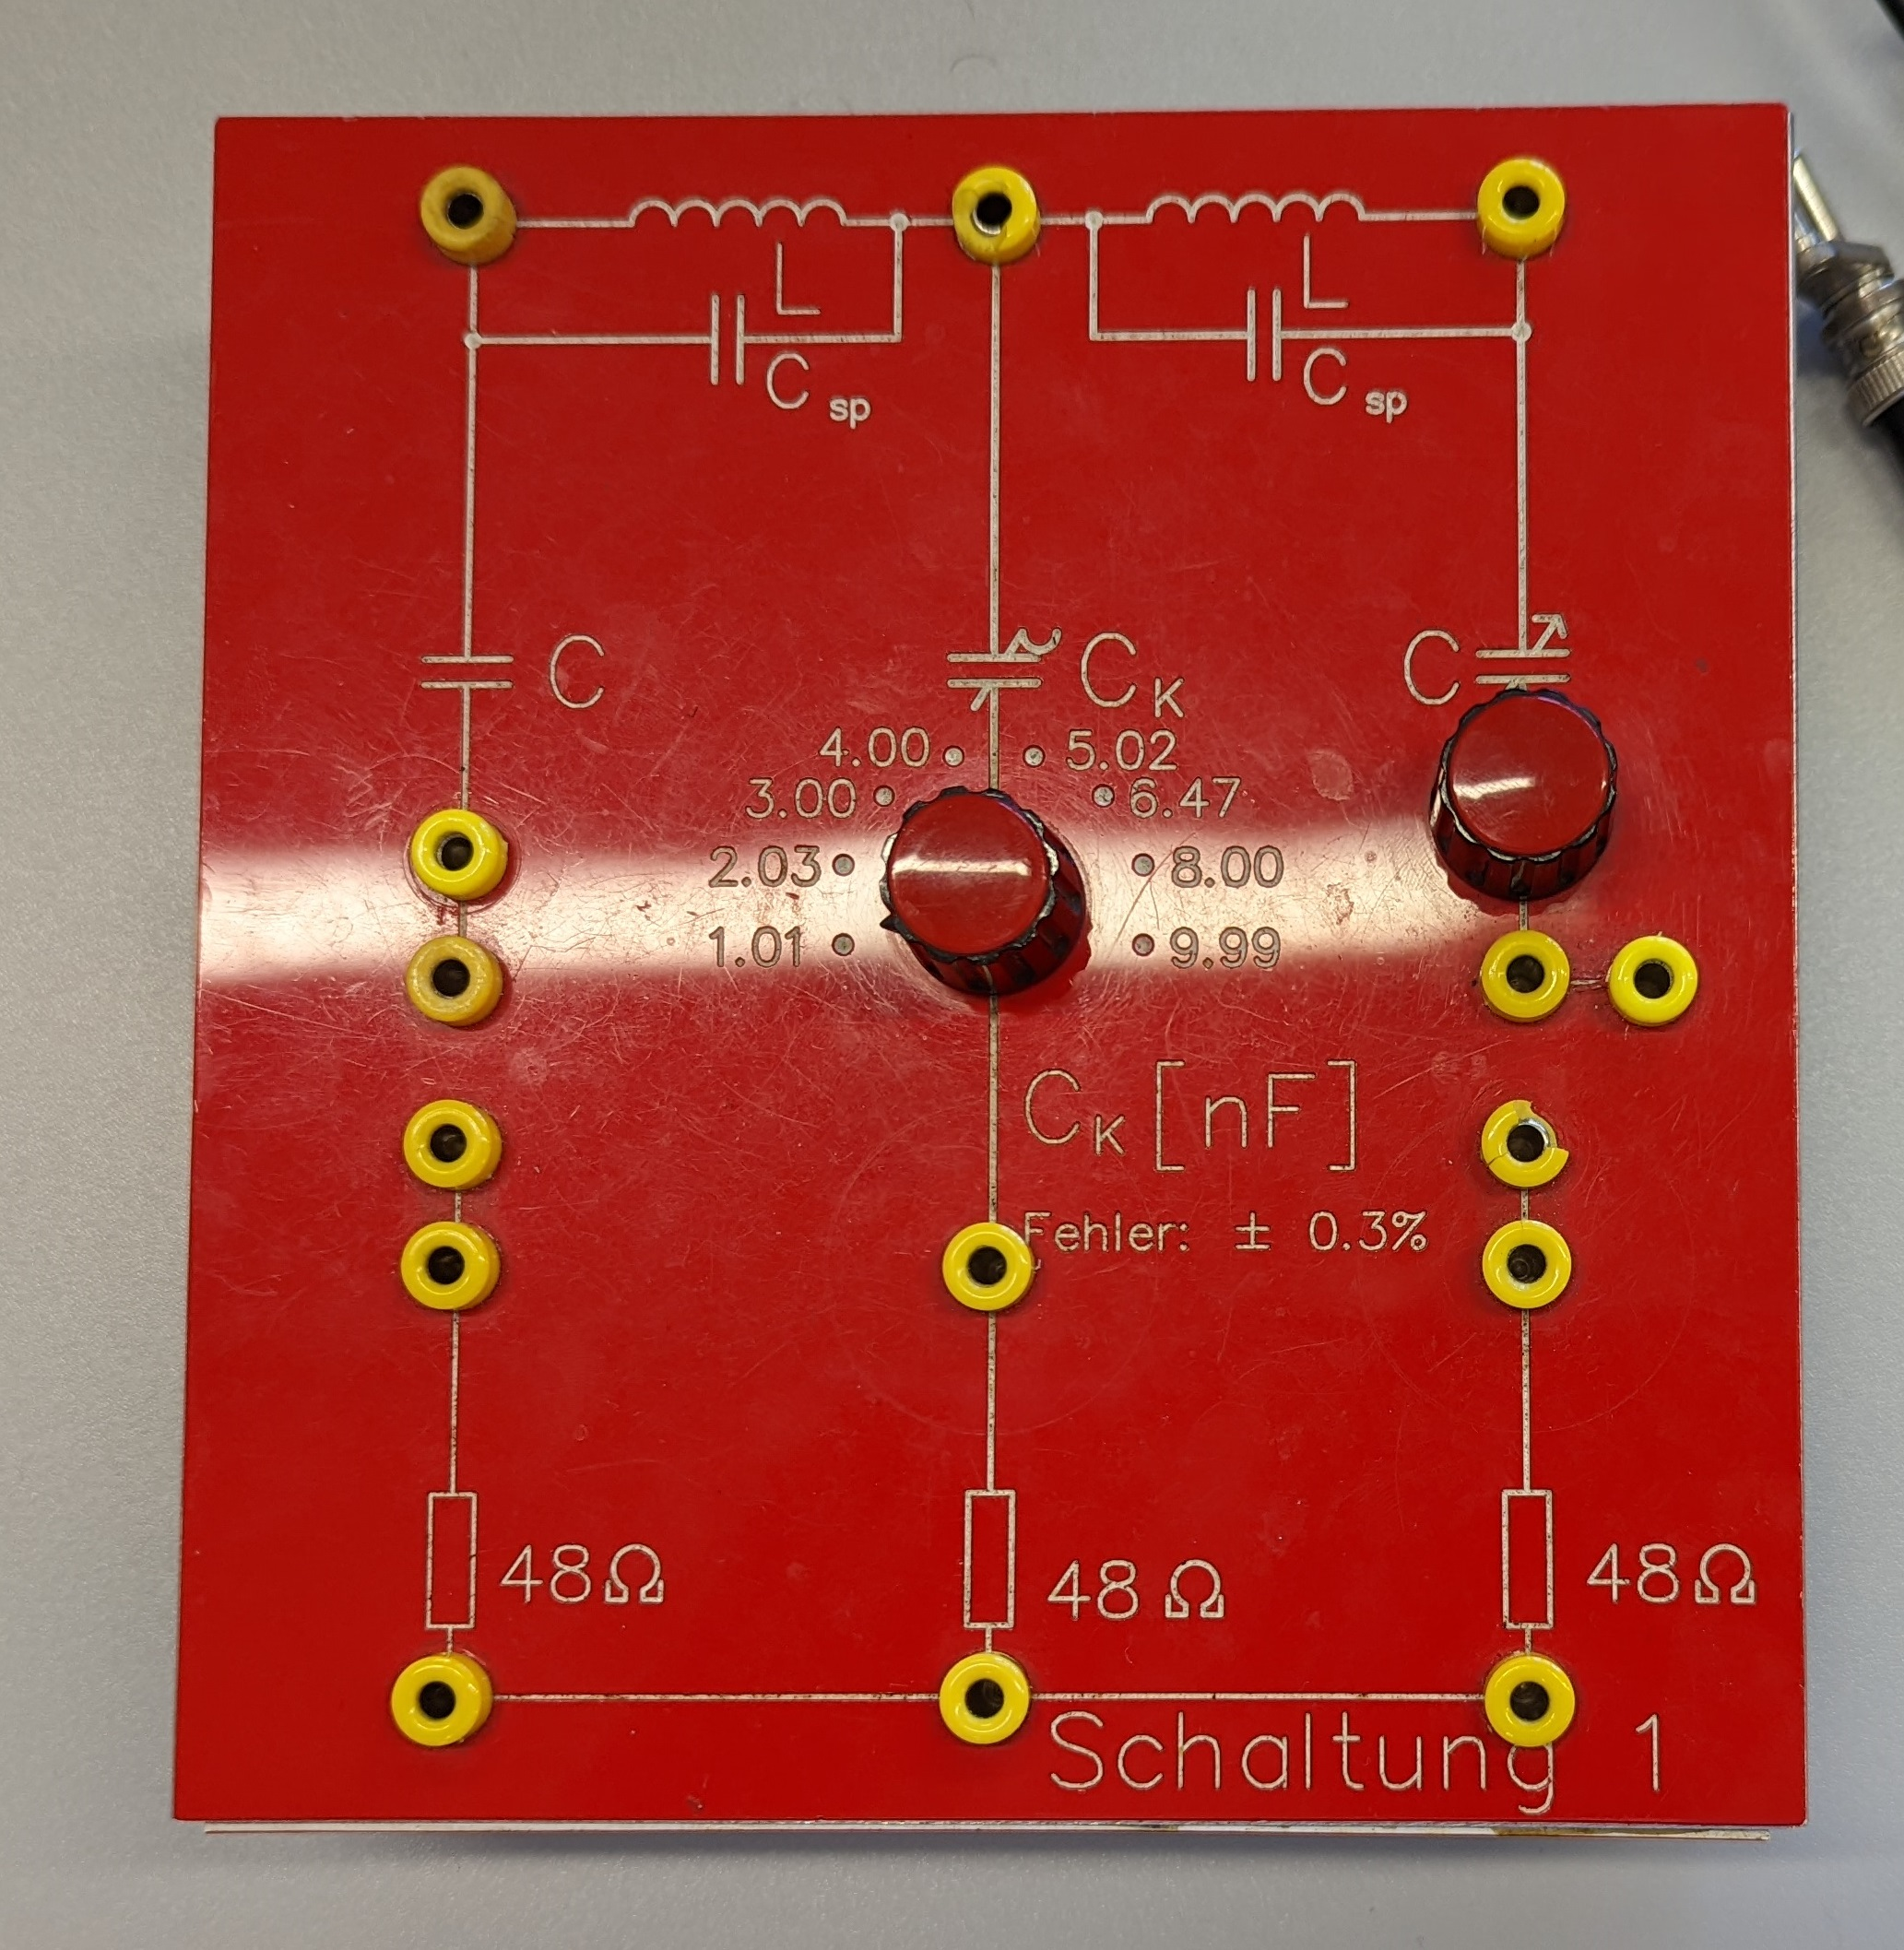
\includegraphics[width=0.5\textwidth]{content/Schaltung.jpg}
\end{figure}

\subsection{Justierung der Resonanzfrequenz}
\label{subsec:Justierung}
Bevor mit dem eigentlichen Messprogramm begonnen werden kann, müssen die beiden Schwingkreise auf die gleiche Resonanzfrequenz abgestimmt werden.
\begin{figure}
    \centering
	\caption{Schaltskizze zur Bestimmung der Resonanzfrequenz \cite{v355}.}
    \label{fig:Schaltung1}
    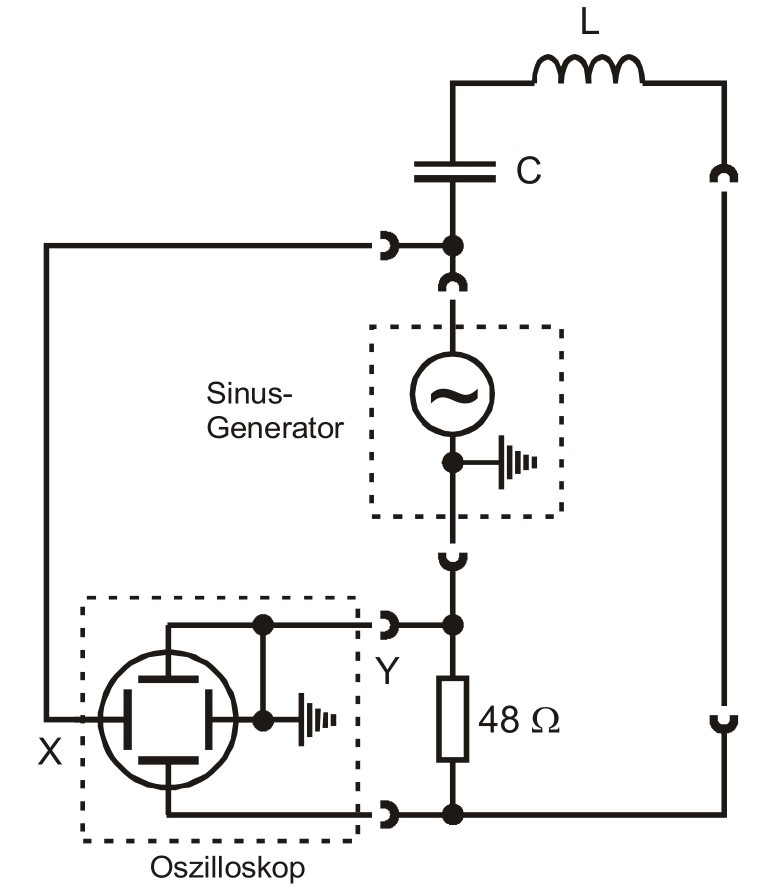
\includegraphics[width=0.5\textwidth]{content/Schaltung1.jpg}
\end{figure}
Dazu wird zuerst die Resonanzfrequenz des linken Schwingkreises festgestellt. Unter Verwendung des Aufbaus aus \autoref{fig:Schaltung1} wird 
der zeitliche Verlauf der am Y-Eingang gemessenen Spannung betrachtet. Durch Variation der Generatorfrequenz wird ein Extremum der Spannung gesucht. Trägt 
man nun die Spannung im Schwingkreis gegen die Generatorspannung auf (XY-Betrieb), entstehen Lissajous-Figuren, anhand derer sich die gesuchte Frequenz genauer
ermitteln lässt. Die Frequenz des Genertors muss dabei so eingestellt werden, dass die Lissajous-Figur eine Gerade darstellt. Die nun eingestellte Frequenz ist
die Resonanzfrequenz. Anschließend wird die Schaltung aus \autoref{fig:Schaltung1} für den rechten Schwingkreis aufgebaut. Mithilfe der regelbaren Kapazität
wird nun die Resonanzfrequenz des Schwingkreises auf die des Linken eingestellt.

\subsection{Messprogramm}
\label{subsec:Messprogramm}
In den folgenden Messungen wird ein Aufbau gemäß \autoref{fig:Schaltung2} verwendet. 
\begin{figure}
    \centering
	\caption{Skizze des Versuchaufbaus \cite{v355}.}
    \label{fig:Schaltung2}
    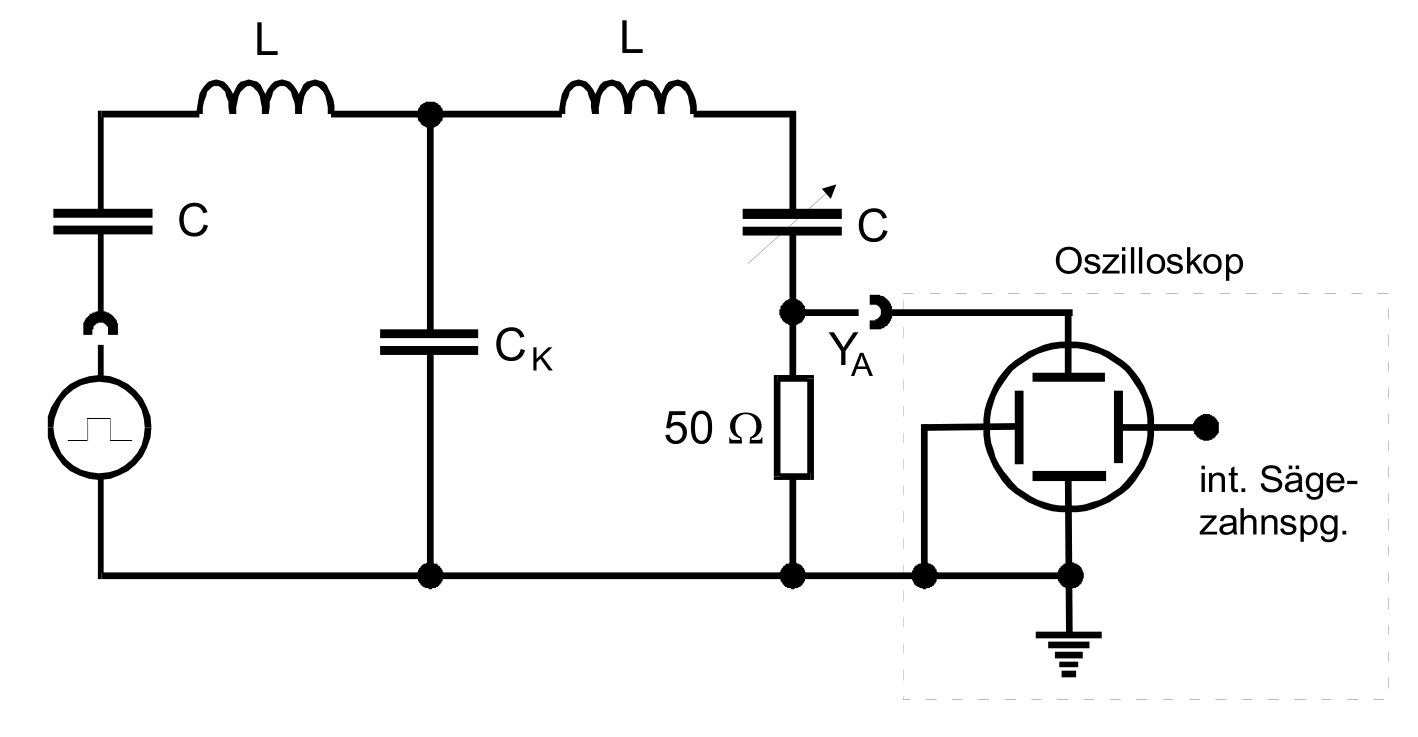
\includegraphics[width=0.7\textwidth]{content/Schaltung2.jpg}
\end{figure}
Um das Verhältnis der Frequenzen von Schwebung und Schwingung zu bestimmen, wird am Generator (links) eine Rechteckspannung mit einer Frequenz von etwa $400\, \unit{\hertz}$
eingestellt. Der zeitliche Verlauf der am $50 \, \unit{\ohm}$ Widerstand abfallenden Spannung kann nun am Oszilloskop entnommen werden. Für die verschiedenen 
Kopplungskondensatoren $C_K$ wird die Anzahl der Schwingungsmaxima innerhalb einer Schwebungsperiode notiert.

Im zweiten Teil der Messung wird der Rechteckimpuls des Generators durch eine Sinusschwingung ersetzt. Als Ausgangsfrequenz wird die Resonanzfrequenz des Schwingkreises
gewählt. Durch Auftragen der am $Y_A$-Eingang gemessenen Spannung gegen die Generatorspannung entstehen Lissajous-Figuren auf der Anzeige des Oszilloskops. Die beiden 
Frequenzen bei denen sich eine Gerade einstellt sind die Frequenzen $\nu^+$ und $\nu^-$ der Fundamentalschwingungen. Ihre Werte werden in Abhängigkeit zur Kapazität 
des Kopplungskondensators notiert.

Im letzten Teil der Messung soll die Frequenzabhängigkeit des Stroms gemessen werden. Dazu wird die \textit{Sweep}-Funktion des Spannungsgenerators genutzt. Mit dieser
lässt sich ein einstellbares Frequenzspektrum durchlaufen. Als Startwert sollte $20 \, \unit{\kilo\hertz}$- und als Endwert $50 \, \unit{\kilo\hertz}$ gewählt werden. Die Zeit 
in der dieser Frequenzbereich durchlaufen wird sollte auf $0.02 \, \unit{\second}$ eingestellt werden. Auf dem Bildschirm des Oszilloskops entsteht nun ein Spannungsverlauf,
an dem zwei große Peaks zu erkennen sind, die den Fundamentalfrequenzen $\nu^+$ und $\nu^-$ entsprechen. Es werden die Breite einer Periode des Verlaufes, der Zeitpunkt an
denen die Maxima auftreten und der Betrag der Maxima notiert. Dies wird für alle Kondensatoren $C_K$ wiederholt.
